\section{Introduction}
\label{sec:intro}

In order for an agent to operate in a dynamic environment, the agent
needs to be constantly observing the external world so that it can
keep up to date with how the world is changing. Therefore, a robotic
agent needs to be planning in situ so that it can alter, or update,
its plan according to the changes. The actual execution of the plan
will also need to change accordingly. The execution also provide
constant feedback on how the world is evolving. Thus as a result of
the dynamic environment, the robotic agent will need to anticipate
constant changes in the plan and need to evaluate how to properly
execute the plan.

In the pursuit of planning in a dynamic environment, earlier work done
in \texttt{IPEM} \cite{AmbrosIngerson88}, \texttt{ROGUE}
\cite{Haigh98}, and the LAAS Architecture \cite{alami:1998p820} have
all helped to make real-world planning possible. Based on these past
successes, there have been multiple experiments that have successfully
functioned in the real-world, the Remote Agent Experiment \texttt{RAX}
\cite{mus98} and the Autonomous Spacecraft Experiment \texttt{ASE}
\cite{chien99}. In particular, we focus on constraint-based temporal
planning which has been demonstrated to be a viable solution for
real-world planning (citation).
	
\fcomment{I need to rework the following section, started here}
At the highest level of abstraction, constraint-based temporal
planning uses a temporal plan to organize how the world works. A
temporal plan is made up of multiple timelines which each describe the
evolution of a subsystem in chronological order. An example of a
subsystem would be the navigator for a robotic agent. Each timeline is
simply the encapsulation of all the possible state values for a
subsystem, within the parameters of a plan.  Therefore, a timeline can
be broken down into its state values along with their temporal
extents, which are defined as tokens. As the base unit for a timeline,
tokens describe the simplest behavior of a subsystem e.g. turn
right. THis kind of representation as it follows least commitment
planning strategy. It herefore allow to have a plan which is partailly
grounded and especially tokens star, duration anfd end times are
represented as intervals depiciting all the acceptable values for
each. By doing so this leave  mroe flexiblity during execution to
decided when -- within the specified domains -- an event should
occur accroding to the current context. This also raises the probelem
that thids decision should then be taken after the plan was produced
by the executive. A lot of exitiing work ahas been made in the area on
the best approach to send the plan to dispach the produced plan to an
executive so it is easier for it to maintin the temporla constraints
within this plan at execution (references). This still leave an issue
open : how does one decide at execution whether a plan actitivy (or
token) should be started as soon as possible or can be postponed
later. This problem can become imporatnt when you see the plan being
produced within a situated agent. Indeed, while the current set of
objectives fr the agent is known these can evolve as time advance and
the poperators or other agents give it new objectives to be
fullfilled. It becomes therefore important for the agent to be
proactive when required while being able to disitinguish actions that
are not yet urgent. We propose here a systematic  approach to allow
the agent to distinguishe which part of the plan needs to be taken
proactively by tracing their causal chain within the plan structure.

% It is understood that grounding the start and end times of a
% token decrease the robustness of a robotic agent while in a dynamic
% environment (citations). Therefore, the tokens have flexible intervals
% for their start, duration, and end times.  As an example, the turn
% right behavior could start from a lower bound time of 12pm to an upper
% bound time of 3pm. This means it can start anytime between its lower
% and upper bound, keeping it flexible.  Consequently, it is the agents
% task to choose exactly when to execute such behaviors. We define the
% task of choosing a token and sending it to its appropriate subsystem,
% to be executed, as dispatching.

\paragraph{An Illustrative Example} We define a simple Shopping agent
that will be used to illustrate different approaches and issues that
arise when dispatching. First, the agent can either be at a location or be
traveling. Second, the agent starts with a certain amount of
energy (resource) that will decrease as it travels. Third, the agent has some
actions that allow it to interact with the environment. It can go to a location,
buy items at stores, and eat the edible items for energy. Lastly, the agent can
want to buy an item. In a typical Shopping agent mission,
the goals are to buy a list of items from different stores and be back
home by the end of the night. 

\begin{figure}
  \centering
\subfloat[Domain
illustration]{\label{fig:ex:graph}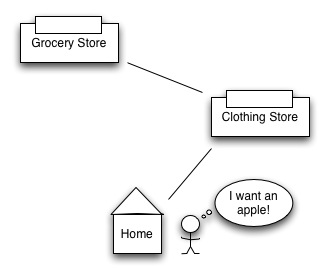
\includegraphics[width=0.51\columnwidth]{figs/example1.jpg}}
\hfill
\subfloat[Initial problem]{\label{fig:ex:init}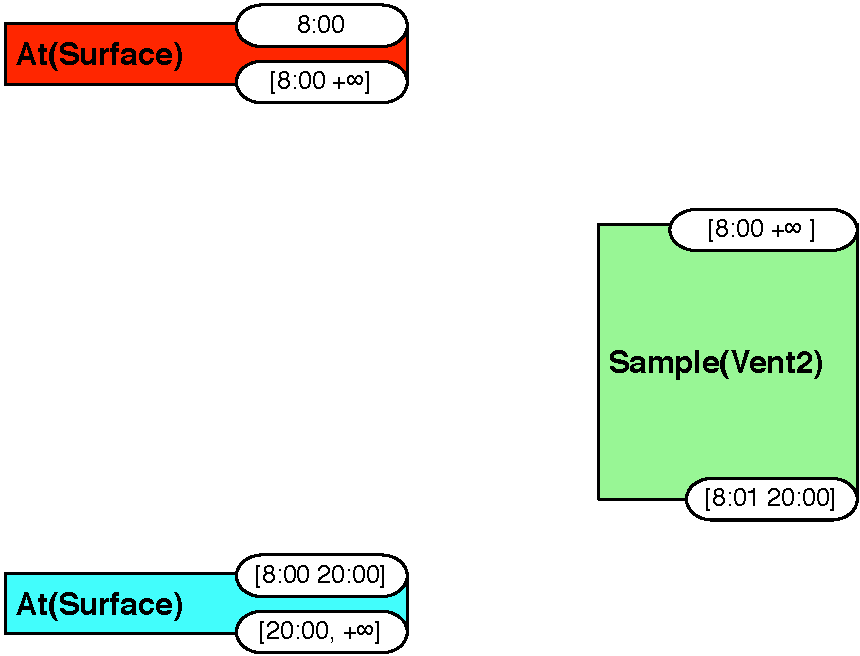
\includegraphics[width=0.47\columnwidth]{figs/example_initial}}
\caption{A description of our shopping agent problem with an
  illustation of the domain (\ref{fig:ex:graph}) along with the intial
  partilal plan for this probelem (\ref{fig:ex:init}). In this domain
  our agent is initially at {\em Home} at 8am, he wants to have an
  {\em Apple}
  before noon and needs to be back 
  at {\em Home} before 8pm (noted 20:00 here).}
\label{fig:Example}
\end{figure}

\begin{figure}
  \centering
  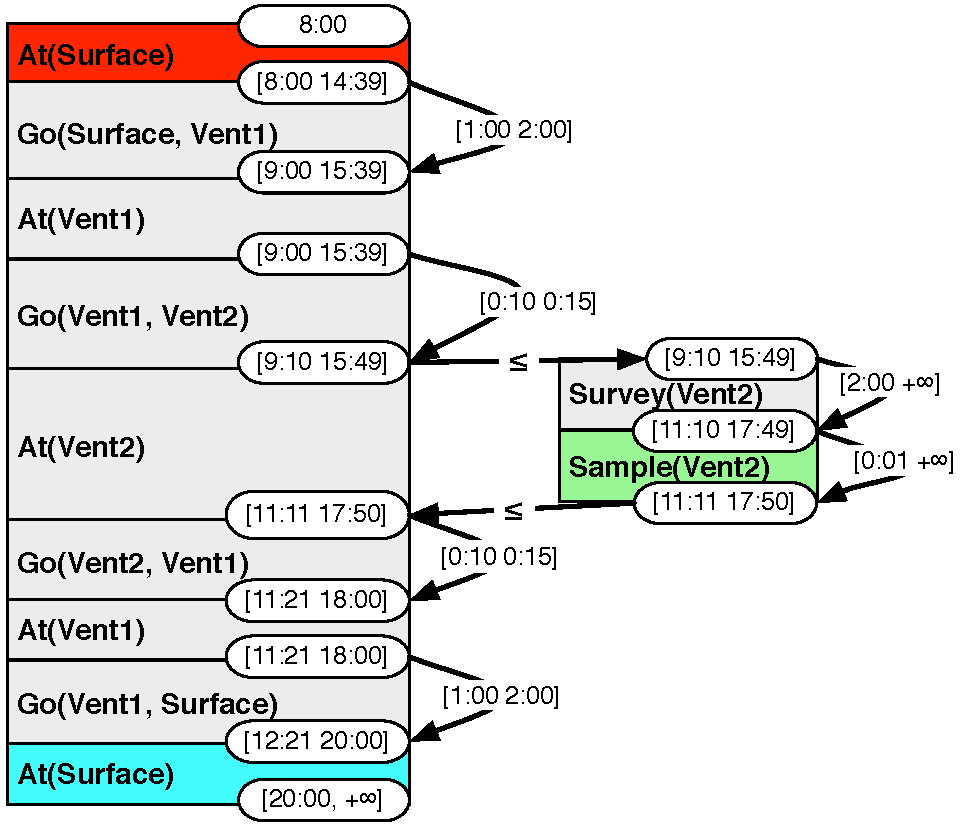
\includegraphics[width=0.8\columnwidth]{figs/example_plan}
  \caption{The felxible plan solution of our domain in
    Fig. \ref{fig:Example}}
  \label{fig:ex:plan}
\end{figure}

However, an issue with finding a balanced approach is deciding whether
it starts to starts its action as early as possible -- which we will
call proactive \fcomment{Need to replace least-commitment by
  ``proactive''}
-- or wait until the action should necessary start --
called later deferred\fcomment{similarly rename EST as ``deferred''}. 
makeThere is a clear difference between the two approaches
 but when should, for example, the shopping agent wait
or start early ? Lets demonstrate an ideal scenario where the shopping
agent balances both approaches. 

The agent, waking up at 8 AM, wants to buy some pants and t-shirts 
and needs to be home by 8 PM. The agent then leaves as early as
possible to start shopping. The agent continues to walk around and 
shop throughout the day because there is no reason to
rush home yet. Around 7 PM, the agent decides that its time to go home
so that it can make it there by 8 PM. What we have demonstrated is a
clear example of how the shopping agent can alternate between the two
approaches depending on the nature of the action or more accurately
the nature of the objective related to this action. Indeed, theagent
was proactive on leaving his house as it was related to him {\em
  wanting}  an apple, on the other hand he just {\em needed} to get
back home by 8 PM allowing him to procrastinate at the grocery 
store. By doing so he will be around in case his wife is calling him
to buy extract things before he gets back home. 

\fcomment{Need a figure that shows the plan somehow ... this can be
  refined as we go along for illustrating proactive vs deferred}

While this example may appear academic at first, it reflects situations
er have seen within embedded agent execution in our domain. Indeed, we
do daily operations wehere our AUV is deployed and scientists can
remotely send new objectives as the mission goes along to the vehicle
as they see new area of interrest. At the same time the vehicle has
also operational objectives such as going to a place wheer its
recovery will be easier for operators. This gives a similar
distinction between the science objectives and operation
objectives. Similarly to our shopping agent we do not realy want the
AUV to get back to recovery area too early as a new science goal could
be sent to him which in turns would rather be fulfilled as early as
possible.

This paper discusses the problem of dispatching when trying to execute
a plan. In particular, dispatching in a dynamic environment where the
plan is known to change either by uncontrollable events or external
requests with new directives. External requests  can occur
at any time which make them in essence uncontrollable events.
Specifically, we focus on how these new requests, coming from the
external world, will affect the way we dispatch the plan, rather than
how they will be integrated into the plan or any part of the planning
process.  The reason for our separation from planning is that
oftentimes planning and executing are split up into two different
jobs. Where a robotic agent is give an already created plan, and it
must then choose how to execute that plan. Therefore, our focus is on
how to dispatch a plan after it has already been created, while
understanding that the plan may still change in the near future.

The approach we have taken on dispatching looks at the token level of a plan,
specifically at the externally requested tokens which we define as goals.
Because they are requested by an external person with the intent of being 
completed, they have a high priority. In contrast, there are tokens that only describe the
evolution of a timeline, which we define as non-goals. In order to keep the plan 
valid, the agent is obligated to complete the non-goals, but there is no rush. Thus, the
non-goals have a low priority. Therefore, we want to complete the goals
as early as possible in order to give adequate time for the possibility of new
goals, and complete the non-goals as they become necessary for the validity of the plan. 
Some may argue that finishing the goals early doesn�t guarantee that
there will be enough time for new goals, however, that is an issue with planning, 
and our concern is with dispatching.


%%% Local Variables: 
%%% mode: latex
%%% TeX-master: "aaai13"
%%% End: 
